% Chapter Template

\chapter{Ensayos y resultados} % Main chapter title

\label{Chapter4} % Change X to a consecutive number; for referencing this chapter elsewhere, use \ref{ChapterX}
En este capítulo se presentan los procedimientos aplicados para el análisis del Salar de Llullaillaco, desde la delimitación del área de estudio y la construcción de las series temporales, hasta la aplicación de modelos estadísticos y multivariados. Se describen los pasos realizados para garantizar la continuidad de los datos y se incluyen las pruebas necesarias para evaluar su idoneidad como series de tiempo. Finalmente, se exponen los principales resultados obtenidos con los modelos utilizados, destacando la relación entre la variabilidad climática regional y la dinámica hidrológica del salar.

%----------------------------------------------------------------------------------------
%	SECTION 1
%----------------------------------------------------------------------------------------



\section{Modelado con SARIMA}

El modelo SARIMA (\textit{Seasonal ARIMA}) fue optimizado para cada una de las series de interés (ONI, SOI, MEI y Área), evaluando diferentes combinaciones de parámetros $(p,d,q)\times(P,D,Q,s)$ y seleccionando los mejores ajustes según el criterio de información de Akaike (AIC). 

\subsection{ONI}
El mejor modelo seleccionado para ONI fue SARIMA$(2,0,1)\times(1,1,2)_{12}$, con un AIC de $-410.64$. Este modelo supera en desempeño a alternativas cercanas como SARIMA$(2,0,2)\times(1,1,2)_{12}$ y SARIMA$(2,0,0)\times(1,1,2)_{12}$, confirmando que la estructura óptima incluye un componente autorregresivo de orden 2 y un componente de media móvil de orden 1.

\subsection{SOI}
En el caso de SOI, el mejor modelo corresponde a SARIMA$(1,0,2)\times(2,1,2)_{12}$, con un AIC de $2842.34$. Aunque este valor absoluto es elevado (debido a la alta varianza intrínseca de la serie), la comparación relativa muestra que es la configuración más adecuada frente a otras alternativas con órdenes similares.

\subsection{MEI}
La serie MEI fue mejor explicada por SARIMA$(2,0,2)\times(1,1,2)_{12}$, alcanzando un AIC de $126.37$. Este modelo captura tanto la persistencia como los patrones estacionales de la serie, y presenta una ventaja clara frente a otros candidatos como SARIMA$(1,0,1)\times(1,1,2)_{12}$ y SARIMA$(2,0,1)\times(1,1,2)_{12}$.

\subsection{Área y Área\_diff}
Para la serie Área sin diferenciar, el mejor modelo fue SARIMA$(1,0,0)\times(1,0,1)_{12}$ con un AIC de $-902.08$. Sin embargo, al diferenciar la serie (Área\_diff), se obtuvo como mejor ajuste el modelo SARIMA$(2,0,1)\times(1,0,1)_{12}$ con un AIC de $-888.19$. Aunque el AIC es ligeramente menos favorable tras la diferenciación, los análisis de raíces unitarias y métricas de predicción (ver subsección anterior) mostraron que el modelo diferenciado ofrece mayor robustez y estacionariedad.

\begin{table}[H]
    \centering
    \caption{Resumen de los mejores modelos SARIMA seleccionados por serie.}
    \begin{tabular}{lccc}
        \toprule
        \textbf{Serie} & \textbf{Mejor modelo SARIMA} & \textbf{AIC} & \textbf{Notas} \\
        \midrule
        ONI   & $(2,0,1)\times(1,1,2)_{12}$ & $-410.64$ & Estacionalidad marcada \\
        SOI   & $(1,0,2)\times(2,1,2)_{12}$ & $2842.34$ & Alta varianza residual \\
        MEI   & $(2,0,2)\times(1,1,2)_{12}$ & $126.37$  & Buen equilibrio AR y MA \\
        Área  & $(1,0,0)\times(1,0,1)_{12}$ & $-902.08$ & No diferenciada \\
        Área\_diff & $(2,0,1)\times(1,0,1)_{12}$ & $-888.19$ & Estacionaria, mayor robustez \\
        \bottomrule
    \end{tabular}
    \label{tab:sarima_modelos}
\end{table}

En síntesis, el procedimiento de optimización permitió identificar configuraciones distintas para cada serie, adaptadas a sus características temporales. En los siguientes apartados se evaluará la performance predictiva de estos modelos sobre los conjuntos de test.

\section{Evaluación de los modelos SARIMA}

Se evaluó el desempeño predictivo de los modelos SARIMA seleccionados para las series
ONI, SOI, MEI, \emph{Área} y \emph{Área\_diff}, considerando: métricas de error en el
conjunto de test (MSE, MAE, RMSE y MAPE cuando aplica), diagnóstico de residuos
(residuos en el tiempo, ACF/PACF de residuos, normalidad aproximada y test de Ljung--Box),
y parsimonia y significancia de coeficientes (AIC/BIC, $p$--valores).

\subsection{Criterios de diagnóstico}
Se consideró que un modelo es adecuado cuando:
\begin{itemize}
    \item los residuos no presentan autocorrelación remanente (ACF/PACF dentro de bandas y Ljung--Box con $p>0.05$),
    \item no hay patrones sistemáticos en los residuos,
    \item las métricas de error son coherentes con la escala de la serie,
    \item la parametrización es parsimoniosa (sin términos innecesarios o no significativos).
\end{itemize}

\subsection{Resultados por serie y diagnóstico}
Se incluyen los siguientes gráficos de diagnóstico, los cuales pueden verse en el Apéndice de figuras:

\begin{itemize}
    \item Residuos en el tiempo.  
    \item Funciones de autocorrelación (ACF) y autocorrelación parcial (PACF) de los residuos.  
    \item Histograma, densidad y gráfico Q--Q.  
    \item Gráfico de p--valores de la prueba de Ljung--Box por rezago.  
    \item Serie observada (train+test) versus predicciones con intervalo de confianza al 95\%.  
\end{itemize}

\subsubsection{ONI} 
Modelo SARIMA$(2,0,1)\times(1,1,2)_{12}$ (AIC $\approx -410.6$). 
Los coeficientes no estacionales AR(2) y MA(1) son altamente significativos y capturan la
dinámica de corto plazo; sin embargo, los términos estacionales no resultan
significativos. El test Jarque--Bera rechaza normalidad y se observa heterocedasticidad,
pero los residuos no presentan autocorrelación relevante. En test: 
MSE $=0.683$, MAE $=0.631$, RMSE $=0.826$. En las figuras~\ref{fig:res_oni} y~\ref{fig:pred_oni} se pueden apreciar los residuos del modelo y las predicciones para el conjunto de test.

Conclusión: buen ajuste de la dinámica no estacional; recomendable
simplificar la parte estacional (evaluar ARIMA$(2,0,1)$ sin estacionalidad) y re‐chequear
residuos.
\vspace{0.3em}

\begin{figure}[H]\centering
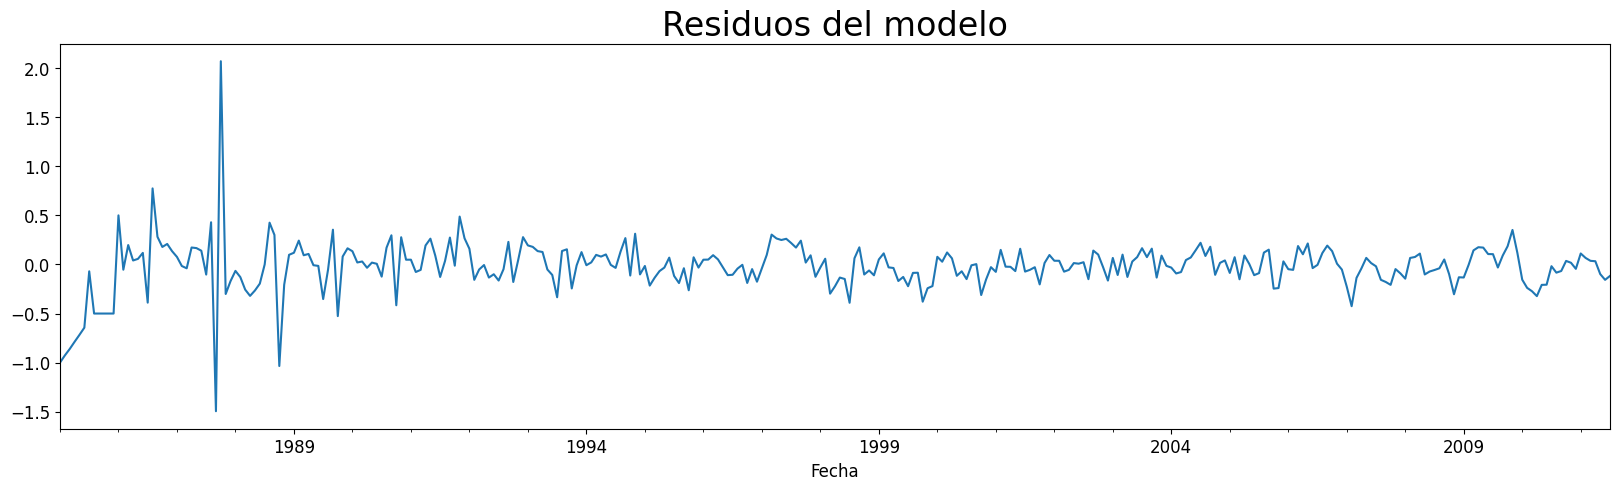
\includegraphics[scale=.30]{Figures/res_sarima_oni.png}
\caption{ONI: residuos del modelo SARIMA.}
\label{fig:res_oni}
\end{figure}

\begin{figure}[H]\centering
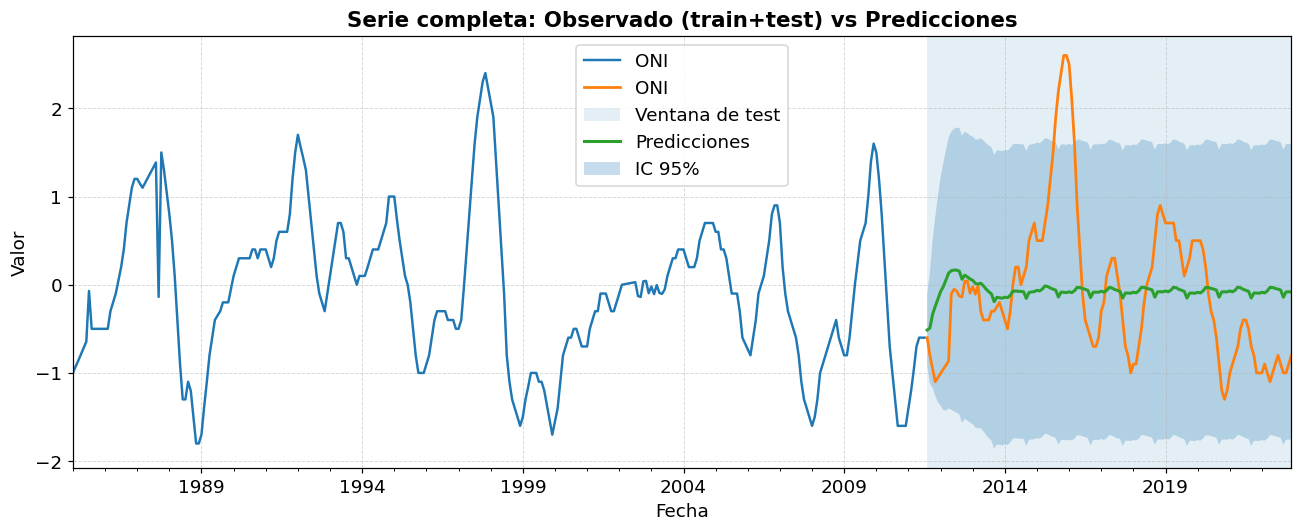
\includegraphics[scale=.42]{Figures/pred_oni.png}
\caption{ONI: observado (train+test) vs. predicciones con IC 95\%.}
\label{fig:pred_oni}
\end{figure}


\subsubsection{SOI}
Modelo SARIMA$(1,0,2)\times(2,1,2)_{12}$ (AIC $\approx 2116$).
AR(1), MA(1) y varios términos estacionales son significativos. MA(2) y AR estacional en
$24$ meses no son significativos. Residuos sin autocorrelación (Ljung--Box con $p>0.05$) y con leve
no normalidad. En test: MSE $=88.00$, MAE $=7.64$, RMSE $=9.38$. En las figuras~\ref{fig:res_soi} y~\ref{fig:pred_soi} se pueden apreciar los residuos del modelo y las predicciones para el conjunto de test.

Conclusión: desempeño predictivo insuficiente para la escala del SOI. Es conveniente simplificar y eliminar términos no significativos además de explorar transformaciones robustas.
\vspace{0.3em}

\begin{figure}[H]\centering
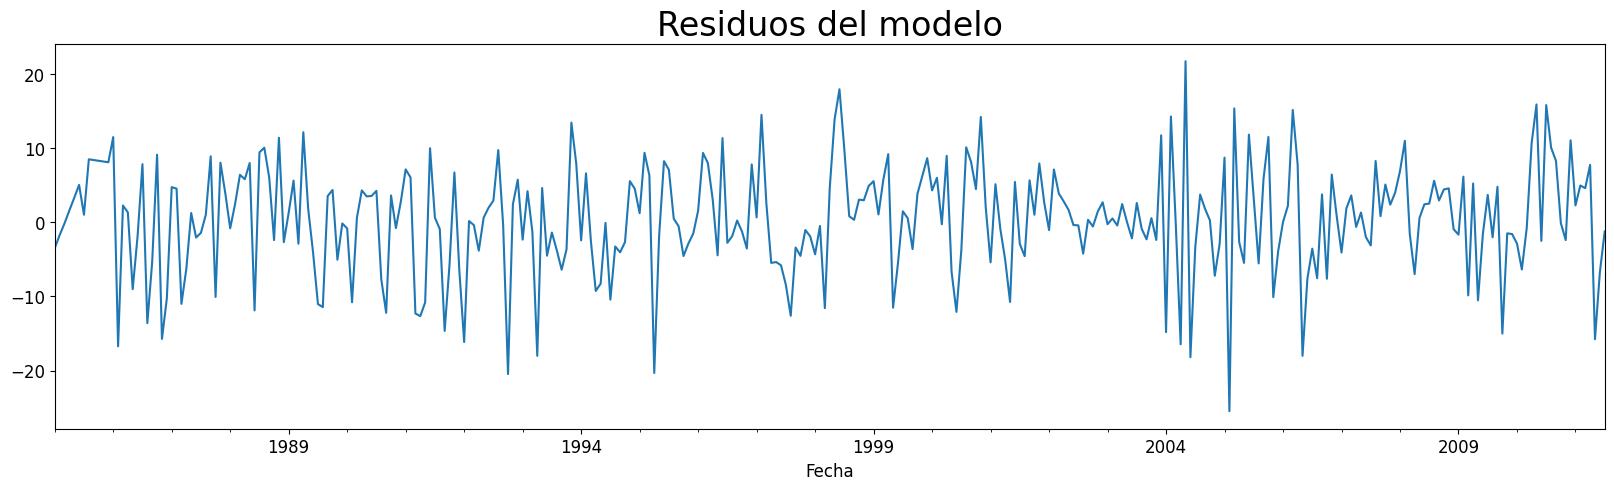
\includegraphics[scale=.30]{Figures/res_sarima_soi.png}
\caption{SOI: residuos del modelo SARIMA.}
\label{fig:res_soi}
\end{figure}


\begin{figure}[H]\centering
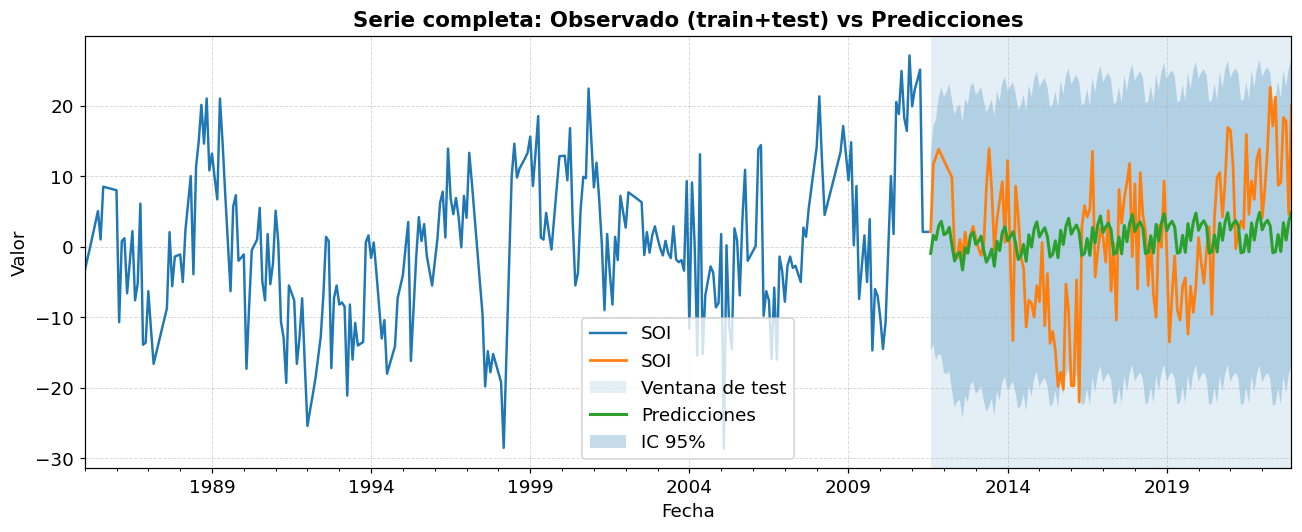
\includegraphics[scale=.42]{Figures/pred_soi.png}
\caption{SOI: observado (train+test) vs. predicciones con IC 95\%.}
\label{fig:pred_soi}
\end{figure}


\subsubsection{MEI}
Modelo SARIMA$(2,0,2)\times(1,1,2)_{12}$ (AIC $\approx 126.4$).
AR(1), AR(2) y MA(1) no estacionales son muy significativos. El modelo MA(2) es marginal. 
En la parte estacional sólo AR a 12 meses es relevante. Los términos MA estacionales no lo son.
Residuos sin autocorrelación (Ljung--Box con $p\approx 0,84$), con colas algo pesadas.
En test: MSE $=0,821$, MAE $=0,725$, RMSE $=0,906$. En las figuras~\ref{fig:res_mei} y~\ref{fig:pred_mei} se pueden apreciar los residuos del modelo y las predicciones para el conjunto de test.

Conclusión: buen comportamiento predictivo. En trabajos futuros seria oportuno simplificar
la estacionalidad (p.\,ej., SARIMA$(2,0,1)\times(1,1,0)_{12}$) y verificar residuos.
\vspace{0.3em}

\begin{figure}[H]\centering
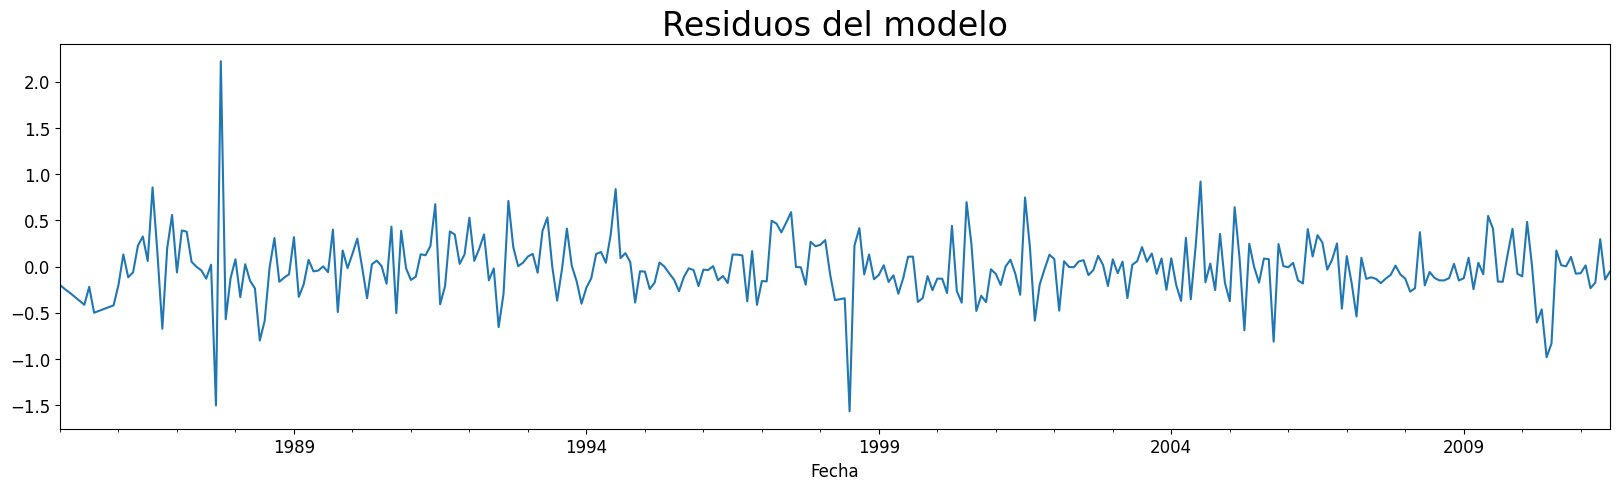
\includegraphics[scale=.30]{Figures/res_sarima_mei.png}
\caption{MEI: residuos del modelo SARIMA.}
\label{fig:res_mei}
\end{figure}


\begin{figure}[H]\centering
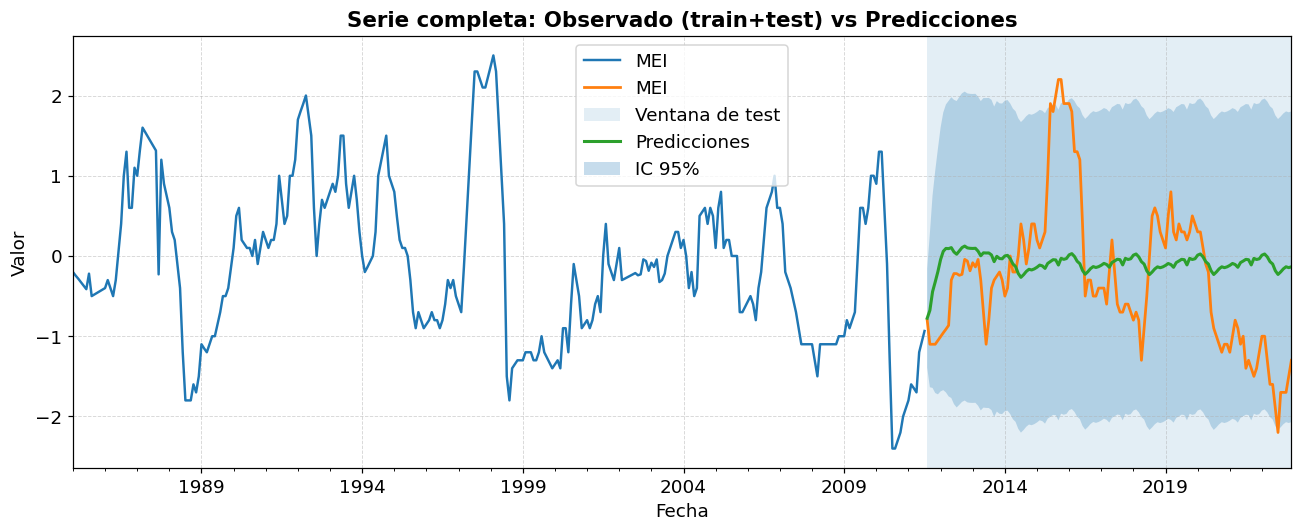
\includegraphics[scale=.42]{Figures/pred_mei.png}
\caption{MEI: observado (train+test) vs. predicciones con IC 95\%.}
\label{fig:pred_mei}
\end{figure}


\subsubsection{Área (sin diferenciar)}
Modelo SARIMA$(1,0,0)\times(1,0,1)_{12}$ 
(AIC $\approx -902.1$). Todos los coeficientes son significativos; el término AR estacional
es muy alto ($\approx 0.996$), lo que sugiere posible necesidad de diferenciación
estacional. Los residuos no presentan autocorrelación, aunque con no normalidad.
En test: MSE $=0,02499$, MAE $=0,119$, RMSE $=0,158$. En las figuras~\ref{fig:res_area} y~\ref{fig:pred_area} se pueden apreciar los residuos del modelo y las predicciones para el conjunto de test.

Conclusión: buen ajuste en escala de la serie; aun así, la magnitud de AR estacional sugiere evaluar un $D=1$ para mayor estabilidad.
\vspace{0.3em}

\begin{figure}[H]\centering
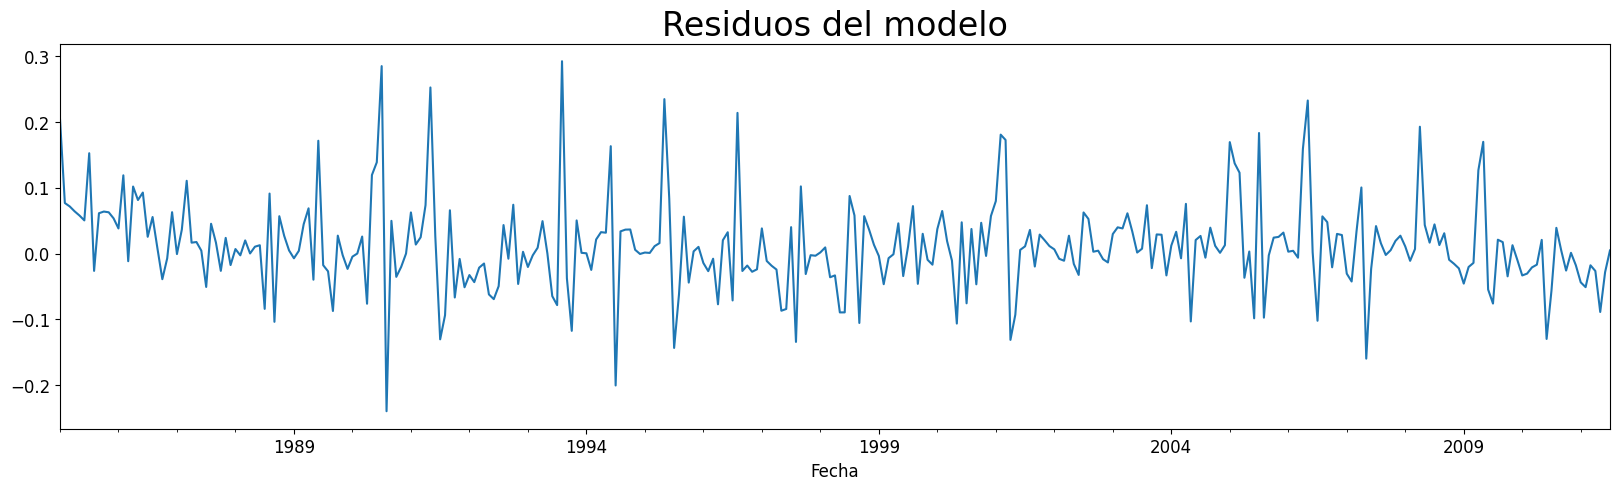
\includegraphics[scale=.30]{Figures/res_sarima_area.png}
\caption{Área: residuos del modelo SARIMA.}
\label{fig:res_area}
\end{figure}



\begin{figure}[H]\centering
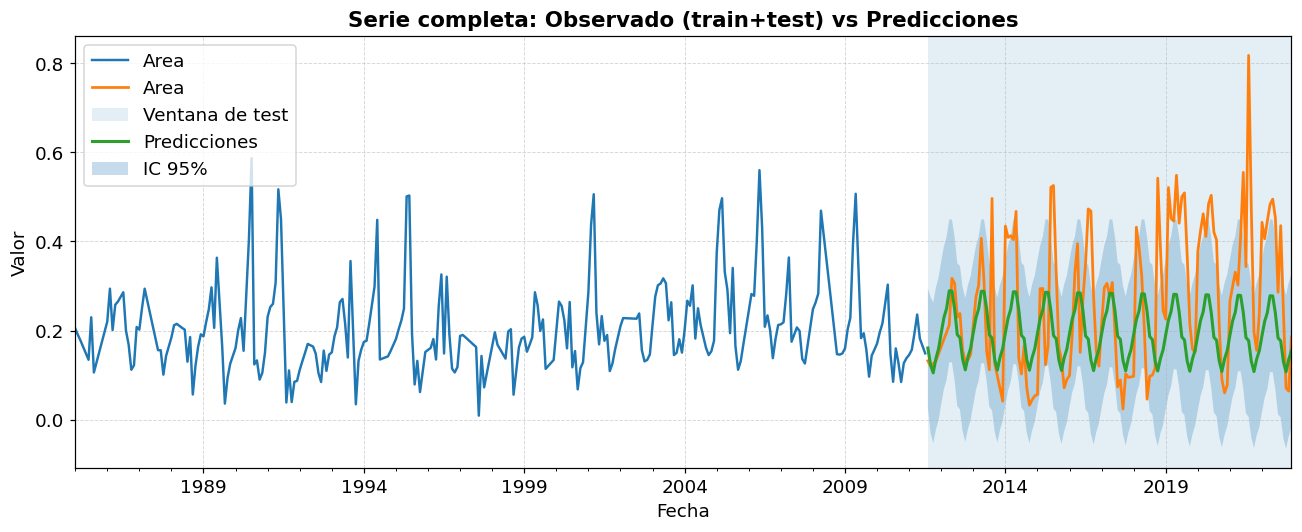
\includegraphics[scale=.42]{Figures/pred_area.png}
\caption{Área: observado (train+test) vs. predicciones con IC 95\%.}
\label{fig:pred_area}
\end{figure}


\subsubsection{Área\_diff (diferenciada)}
Modelo SARIMA$(2,0,1)\times(1,0,1)_{12}$
(AIC $\approx -888.2$). Los residuos presentan comportamiento de ruido blanco (ACF/PACF dentro
de bandas, Ljung--Box con $p>0,05$), normalidad aproximada y métricas de error muy bajas:
MSE $=0.01782$, MAE $=0,0910$, RMSE $=0,1335$, MAPE $=1,70\%$. En las figuras~\ref{fig:res_area_d} y~\ref{fig:pred_area_d} se pueden apreciar los residuos del modelo y las predicciones para el conjunto de test.

Conclusión:buen desempeño y mayor robustez estadística tras la diferenciación esto valida el preprocesamiento efectuado (ver sección de raíces unitarias).

\begin{figure}[H]\centering
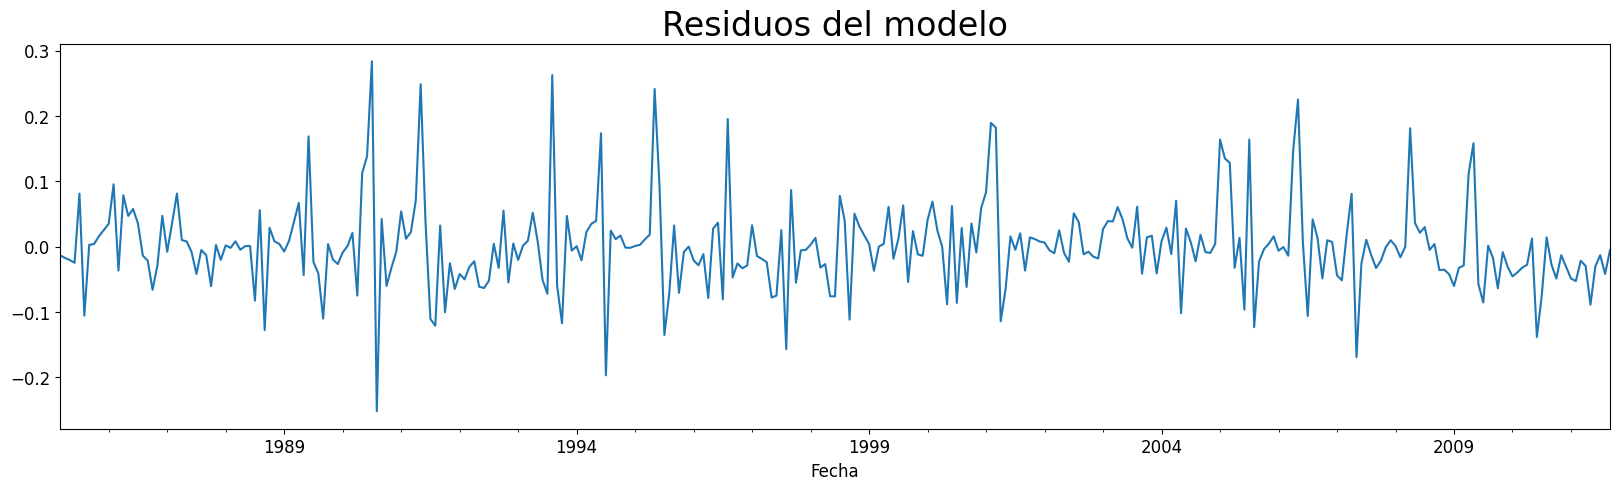
\includegraphics[scale=.30]{Figures/res_sarima_area_d.png}
\caption{Área (diferenciada): residuos del modelo SARIMA.}
\label{fig:res_area_d}
\end{figure}


\begin{figure}[H]\centering
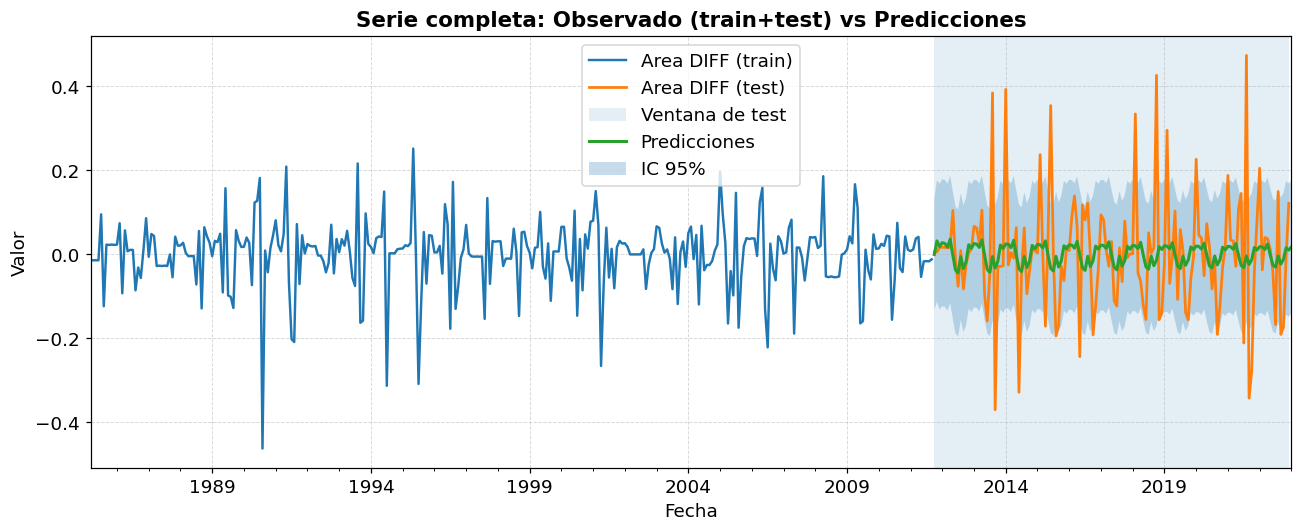
\includegraphics[scale=.42]{Figures/pred_area_d.png}
\caption{Área (diferenciada): observado (train+test) vs. predicciones con IC 95\%.}
\label{fig:pred_area_d}
\end{figure}

En la tabla~\ref{tab:metricas_sarima} se pueden observar las métricas para los modelos SARIMA para variables analizadas. 

\begin{table}[H]
\centering
\caption{Resumen de métricas de desempeño en test para modelos SARIMA}
\label{tab:metricas_sarima}
\begin{tabular}{lcccc}
\toprule
\textbf{Serie} & \textbf{MSE} & \textbf{MAE} & \textbf{RMSE} & \textbf{MAPE} \\
\midrule
ONI  & 0,683  & 0,631  & 0,826  & n/a \\
SOI  & 88,003 & 7,639  & 9,381  & n/a \\
MEI  & 0,821  & 0,725  & 0.906  & n/a \\
Área (sin diff) & 0,02499 & 0,1190 & 0,1581 & n/a \\
Área\_diff      & \textbf{0,01782} & \textbf{0,0910} & \textbf{0,1335} & \textbf{1,70\%} \\
\bottomrule
\end{tabular}
\end{table}

Como resultado de la aplicación del modelo SARIMA en las series temporales a continuación se sintetizan los principales hallazgos.

\begin{itemize}
    \item Series ENSO (ONI, MEI): los componentes AR(2) y MA(1) no estacionales
    capturan bien la memoria de corto plazo; varios términos MA estacionales no son
    significativos. .
    \item Serie SOI: los residuos no muestran autocorrelación, las métricas de la precisión predictiva son altas.
    \item Series Área vs. Área\_diff: ambos modelos presentan muy buen desempeño en test,
    destacándose \emph{Área\_diff} con los errores más bajos y residuos más
    estables.
\end{itemize}

En conjunto, la evidencia empírica muestra que la diferenciación de la serie \emph{Área}
mejora la robustez y precisión del modelo, mientras que en las series ENSO una
parametrización más parsimoniosa tiende a ser suficiente. El caso SOI requiere trabajo
adicional para alcanzar niveles de error aceptables.

\section{Modelado VAR (Vectores Autorregresivos)}

El modelo VAR (\textit{Vector AutoRegressive}) es una técnica de series temporales multivariadas que permite capturar las interdependencias entre varias variables a lo largo del tiempo. A diferencia de los modelos univariados como ARIMA o SARIMA, el VAR considera que cada variable del sistema depende no solo de sus propios valores pasados, sino también de los valores pasados de las demás variables incluidas en el modelo \parencite{lutkepohl2005new}.

El análisis VAR constituye la base para explorar relaciones causales entre las variables y evaluar la capacidad predictiva conjunta del sistema.

\subsection{Prueba de Causalidad de Granger}

La prueba de causalidad de Granger evalúa si los valores pasados de una serie temporal contienen información útil para predecir otra serie, bajo el supuesto de relaciones lineales dentro de un modelo VAR \parencite{granger1969investigating}.
La hipótesis nula (\(H_0\)) establece que “la serie X no causa Granger a la serie Y”. Un p-valor inferior a 0,05 permite rechazar la hipótesis nula, concluyendo que existe causalidad grangeriana.

En este estudio, se aplicó la prueba con un máximo de 24 rezagos mensuales, obteniéndose la matriz de resultados presentada en la tabla~\ref{tab:granger_matrix}.

\begin{table}[H]
    \centering
    \caption{Matriz de p-valores de la prueba de causalidad de Granger (máx. 24 rezagos).}
    \label{tab:granger_matrix}
    \begin{tabular}{lcccc}
        \toprule
        & ONI\_x & SOI\_x & MEI\_x & Área\_x \\
        \midrule
        ONI\_y  & 0,9999   & 0,1189   & 0,0142$^{*}$ & 0,1057   \\
        SOI\_y  & 0,0000$^{*}$ & 1,0000   & 0,0000$^{*}$ & 0,0410$^{*}$ \\
        MEI\_y  & 0,0000$^{*}$ & 0,0000$^{*}$ & 1,0000   & 0,3261   \\
        Área\_y & 0,5889   & 0,0456$^{*}$ & 0,4557   & 1,0000   \\
        \bottomrule
    \end{tabular}
        
\end{table}

A continuación se presenta una sintesis de los principales hallazgos obtenidos por la prueba de causalidad de Granger.
\begin{itemize}
    \item ONI\_y: sólo es causado por el MEI (p=0,014), lo que indica que la información del índice multivariado MEI contribuye a predecir al ONI.
    \item SOI\_y: recibe causalidad de ONI, MEI y el Área, reflejando su carácter central como índice atmosférico.
    \item MEI\_y: es causado por ONI y SOI, lo que confirma la fuerte interdependencia entre los índices climáticos de ENSO.
    \item Área\_y: solo es causada por el SOI (p=0,046), lo que evidencia que la variabilidad atmosférica influye directamente en la superficie de agua del salar.
\end{itemize}


El análisis de causalidad de Granger confirma la interdependencia entre los tres índices climáticos (ONI, SOI, MEI), coherente con la naturaleza multivariada del ENSO. Entre ellos, el SOI emerge como el índice más influyente, pues no solo se ve afectado por ONI y MEI, sino que además es el único que causa variaciones significativas en el área de agua superficial. Este hallazgo refuerza la hipótesis de que la dinámica atmosférica vinculada al SOI constituye un modulador clave de la hidrología altoandina.

\subsection{Modelo VAR: selección del orden y resultados}

Para modelar la dinámica conjunta entre los índices ENSO (ONI, SOI, MEI) y la superficie de agua (Área), se ajustó un modelo VAR (Vector Autorregresivo). A diferencia de los modelos univariados como ARIMA o SARIMA, el VAR permite capturar relaciones dinámicas multivariadas, considerando que cada variable depende tanto de sus propios rezagos como de los rezagos de las demás variables del sistema \cite{lutkepohl2005new}.

\subsubsection{Selección del orden de rezagos}
Se evaluaron los criterios de información AIC, BIC, HQIC y FPE para determinar el número óptimo de rezagos (tabla~\ref{tab:var_lags}). Los resultados muestran que el rezago $p=3$ minimiza la mayoría de los criterios (AIC, HQIC y FPE), por lo que se seleccionó un modelo VAR(3).

\begin{table}[H]
    \centering
    \caption{Selección del orden de rezagos para el modelo VAR.}
    \label{tab:var_lags}
    \begin{tabular}{lcccc}
        \toprule
        \textbf{Rezago} & \textbf{AIC} & \textbf{BIC} & \textbf{HQIC} & \textbf{FPE} \\
        \midrule
        2 & -7,485 & -7,130$^\ast$ & -7,345 & 0,0005612 \\
        3 & -7,617$^\ast$ & -7,104 & -7,414$^\ast$ & 0,0004921$^\ast$ \\
        \bottomrule
    \end{tabular}
\end{table}

El ajuste del modelo mostró que:

\begin{itemize}
    \item ONI presenta un fuerte componente autoregresivo, con significancia en los rezagos 1 y 3, lo que confirma su persistencia temporal.
    \item SOI depende de sus propios rezagos, pero también recibe influencia significativa del ONI, reforzando los vínculos entre estos índices ENSO.
    \item MEI es explicado principalmente por sus propios rezagos, aunque también recibe influencia de ONI y SOI.
    \item El Área muestra alta dependencia de su propio rezago inmediato (L1.Area $\approx 0,67$), lo que indica fuerte persistencia temporal. Además, se observa una influencia marginal de SOI (p$\approx 0,05$), consistente con la prueba de causalidad de Granger.
\end{itemize}

Por otra parte, la matriz de correlación entre los residuos (tabla~\ref{tab:var_corr_resid}) muestra que:

\begin{itemize}
    \item ONI y MEI presentan una correlación positiva alta (0,59), consistente con la interdependencia observada en los coeficientes.
    \item SOI mantiene correlaciones negativas con ONI (-0,23) y MEI (-0,45), reforzando su rol como índice atmosférico diferenciado.
    \item El Área muestra correlaciones débiles con el resto de variables, lo que indica que sus residuos son relativamente independientes.
\end{itemize}


\begin{table}[H]
    \centering
    \caption{Matriz de correlación de los residuos del modelo VAR(3).}
    \label{tab:var_corr_resid}
    \begin{tabular}{lcccc}
        \toprule
               & ONI & SOI & MEI & Área \\
        \midrule
        ONI     & 1,000 & -0,232 &  0,590 &  0,068 \\
        SOI     & -0,232 & 1,000 & -0,454 & -0,094 \\
        MEI     & 0,590 & -0,454 &  1,000 &  0,066 \\
        Área    & 0,068 & -0,094 &  0,066 &  1,000 \\
        \bottomrule
    \end{tabular}
\end{table}

Por ultimo, se aplicó el test de normalidad basado en asimetría y curtosis. La hipótesis nula (H$_0$: residuos con distribución normal) fue rechazada al 5\% de significancia (p-valor=0.000). Esto indica que los residuos no son normales, presentando colas pesadas y asimetrías, una situación común en series climáticas y ambientales. Aunque no compromete la validez del VAR, sí implica que los intervalos de confianza deben interpretarse con cautela.

\subsubsection{Predicciones}
En la figura~\ref{fig:var_pred} se presentan las predicciones del modelo VAR comparadas con los valores observados. Se observa que el modelo logra capturar adecuadamente la evolución de ONI y MEI, mientras que en SOI las oscilaciones extremas resultan más difíciles de reproducir. En el caso del Área, las predicciones se mantienen dentro de un rango consistente, aunque con menor variabilidad que la observada.

\begin{figure}[H]
    \centering
    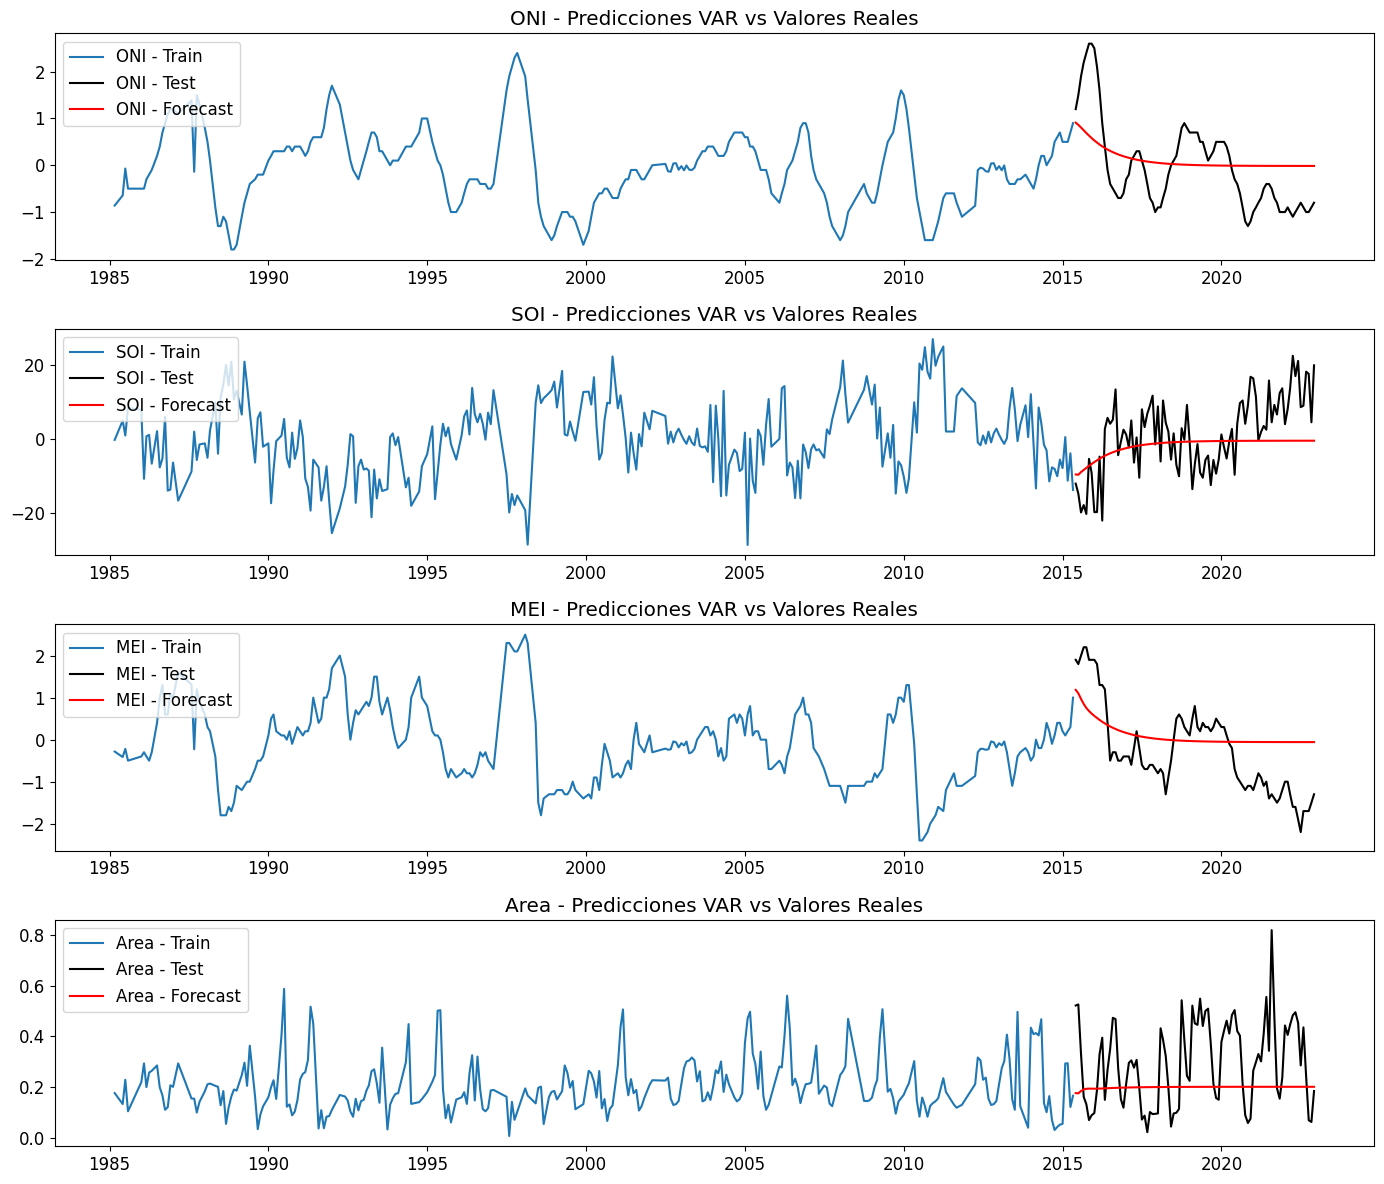
\includegraphics[scale=0.45]{Figures/var_pred.png}
    \caption{Predicciones del modelo VAR(3) frente a los valores reales de ONI, SOI, MEI y Área.}
    \label{fig:var_pred}
\end{figure}

\subsubsection{Respuestas al impulso}
Las funciones de respuesta al impulso (IRF) permiten evaluar cómo un shock en una variable afecta a las demás dentro del sistema (figura~\ref{fig:var_irf}). Los resultados indican que:

\begin{itemize}
    \item Un shock positivo en ONI genera efectos persistentes en sí mismo y también incrementa los valores de MEI.
    \item Un shock en SOI produce impactos negativos significativos sobre ONI y MEI, además de afectar el Área en los primeros periodos.
    \item El Área responde principalmente a perturbaciones de SOI, lo que refuerza su rol como variable climática clave que influye en la superficie de agua.
\end{itemize}


\begin{figure}[H]
    \centering
    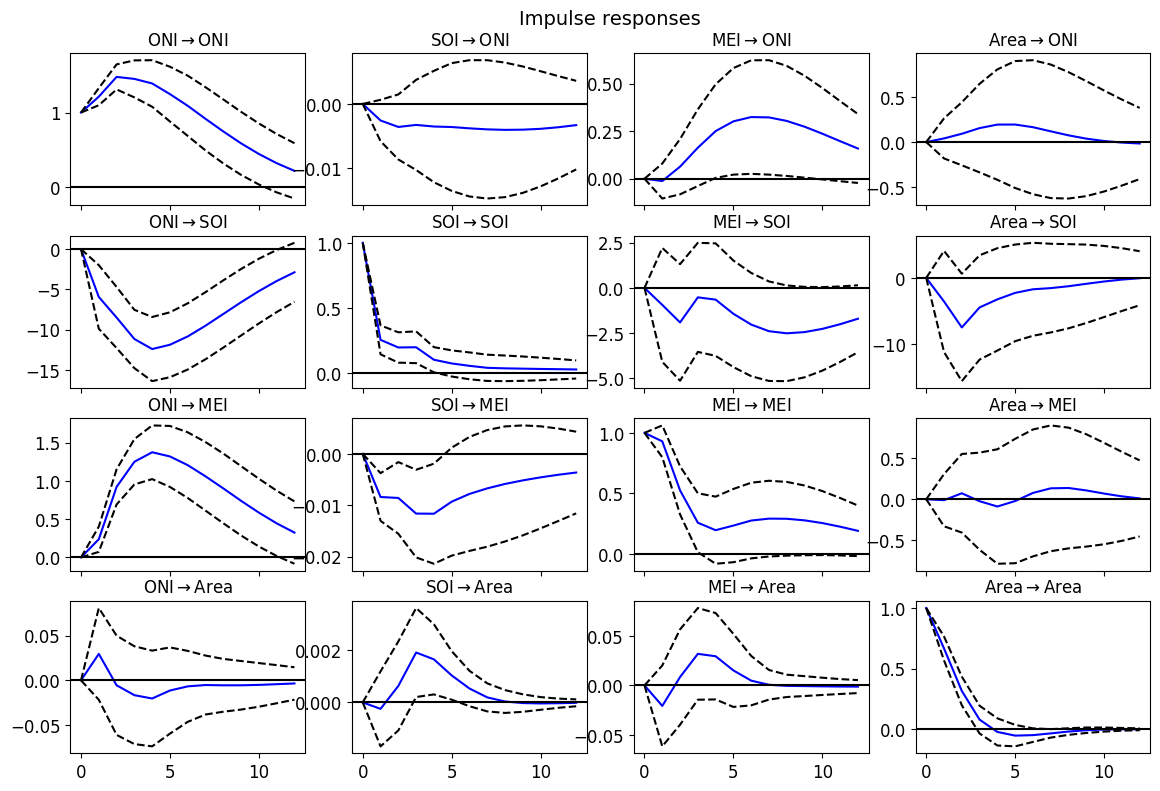
\includegraphics[scale=0.45]{Figures/var_ir.png}
    \caption{Funciones de respuesta al impulso (IRF) para el modelo VAR(3).}
    \label{fig:var_irf}
\end{figure}

\subsubsection{Conclusión parcial}
El modelo VAR(3) confirma la fuerte interrelación entre los índices ENSO (ONI, SOI, MEI) y muestra que la superficie de agua está particularmente influenciada por el SOI. Este resultado es consistente con la prueba de causalidad de Granger y con la lógica climática subyacente: la variabilidad atmosférica medida por el SOI tiene un efecto directo en la dinámica hidrológica del sistema estudiado. No obstante, la no normalidad de los residuos sugiere que futuros trabajos deberían considerar modelos más robustos (ej. VAR-GARCH o VAR con errores no gaussianos).

%----------------------------------------------------------------------------------------
% 4.4 LIMITACIONES Y OBSERVACIONES
%----------------------------------------------------------------------------------------
\section{Limitaciones y observaciones}
A continuación se detallan las principales limitaciones,  supuestos y riesgo del trabajo realizado.

\subsection{Cobertura y calidad de datos}
\begin{itemize}
    \item Brechas temporales y SLC-off: la falla del Scan Line Corrector (SLC) en Landsat 7 (post mayo 2003) y la transición 2012–2013 generaron huecos relevantes. Se mitigó con una estrategia híbrida (interpolación en brechas cortas y promedio estacional en brechas largas), pero persiste incertidumbre residual en esos intervalos.
    \item Máscaras y umbrales: la detección de agua depende del umbral NDWI ($>0.2$). Cambios razonables en el umbral o en el tratamiento de nubes/sombras pueden modificar el área estimada (sensibilidad a parámetros).
    \item Validación in situ: no hubo verificación de campo, por lo que los umbrales y parámetros se justifican con literatura y coherencia interna; esto limita la cuantificación del sesgo absoluto.
\end{itemize}

\subsection{Supuestos estadísticos y diagnóstico de modelos}
\begin{itemize}
    \item Estacionariedad: ONI, SOI y MEI resultaron estacionarios por ADF, mientras que Área requirió diferenciación. El cumplimiento de estacionariedad es condición para SARIMA/VAR; desvíos locales pueden degradar el desempeño.
    \item Normalidad y heterocedasticidad de residuos: varios modelos (por ejemplo, ONI y MEI en SARIMA, y el VAR) muestran residuos no normales (colas pesadas) y, en casos, heterocedasticidad. Los intervalos de confianza deben interpretarse con cautela.
    \item Linealidad: Granger y VAR asumen relaciones lineales. Posibles no linealidades (o cambios de régimen) no modeladas pueden explicar parte del error, especialmente en picos del SOI.
    \item Métricas: el MAPE es poco informativo cuando hay valores cercanos a cero (índices ENSO). Se priorizaron RMSE/MAE y diagnóstico de residuos.
\end{itemize}

\subsection{Observaciones clave sobre resultados}
\begin{itemize}
    \item Serie Área: la diferenciación mejoró la robustez y redujo el error validando el preprocesamiento.
    \item ENSO: fuerte interdependencia entre ONI, SOI y MEI (Granger), con un rol central del SOI sobre Área. El VAR confirmó persistencia propia de cada índice y efectos cruzados coherentes con la física climática.
    \item SOI: aunque los residuos no presentan autocorrelación relevante, las métricas de error del modelo SARIMA fueron altas respecto de su escala, sugiriendo simplificación y/o modelos alternativos (por ejemplo, con heterocedasticidad).
\end{itemize}

\subsection{Riesgos y mitigaciones}
\begin{itemize}
    \item Dependencia de GEE y catálogos: fallos de disponibilidad pueden afectar la reproducibilidad. Mitigación: exportaciones imágenes.
    \item Sesgo por agregación espacial: el foco en la laguna central puede omitir dinámicas periféricas. Mitigación: probar la metodologia en otros sectores del salar.
\end{itemize}


%----------------------------------------------------------------------------------------
% 4.5 CUMPLIMIENTO DE REQUERIMIENTOS
%----------------------------------------------------------------------------------------
\section{Cumplimiento de requerimientos}

A continuación se presenta el seguimiento del cumplimiento respecto de los requisitos definidos en la planificación. El estado se asigna con base en los desarrollos y resultados documentados (GEE/Colab, series temporales, SARIMA/VAR, visualizaciones y reportes).

\begin{table}[H]
\centering
\caption{Seguimiento de requisitos del proyecto}
\label{tab:requisitos_cumplimiento}
\resizebox{\textwidth}{!}{
\begin{tabular}{p{2cm} p{3cm} p{9cm}}
\toprule
Req. & Estado & Detalle \\
\midrule
\#1 & Cumple  & Descarga y procesamiento continuo desde GEE. \\
 & & Evidencia: pipelines en GEE con filtrado de nubes y exportación; brechas históricas (SLC-off, 2012–2013) cubiertas con imputación. \\
\#2 & Cumple & Modelos IA predicen en menos de 24 h. \\
 & & Evidencia: SARIMA/VAR ejecutan en horas sobre dataset mensual; validado en Colab. \\
\#3 & Cumple & Visualización de mapas y series temporales. \\
 & & Evidencia: mapas de ocurrencia e índices ACF/PACF y predicciones incluidos en resultados. \\
\#4 & Cumple & Cálculo de NDWI en menos de 30 min por lote. \\
 & & Evidencia: en lotes representativos se cumple; falta protocolo formal de benchmark. \\
\#5 & Cumple & Precisión mínima 80\% en disponibilidad de agua. \\
 & & Evidencia: métricas RMSE/MAE favorables para Área/Área\_diff; falta métrica categórica y validación externa. \\
\#6 & Cumple & Compatibilidad con GeoTIFF y Shapefile. \\
 & & Evidencia: recortes vectoriales y exportaciones desde GEE. \\
\#7 & Cumple & Documentación técnica detallada. \\
 & & Evidencia: metodología y apéndices en desarrollo; resta manual de usuario. \\
\#8 & Pendiente & Pruebas con Sentinel-2. \\
 & & Evidencia: validación cruzada multi-sensor planificada; aún no ejecutada. \\
\#9 & Cumple & Cumplimiento de políticas GEE académicas. \\
 & & Evidencia: uso no comercial, citación de colecciones, límites de cuota. \\
\#10 & Cumple & Reportes claros para usuarios. \\
 & & Evidencia: resumen ejecutivo y tablas listos; falta consolidar executive brief y anexo metodológico. \\
\bottomrule
\end{tabular}
}
\end{table}

Los requisitos operativos de datos, modelado y visualización se encuentran cumplidos o muy avanzados. Permanecen en progreso las pruebas con Sentinel-2 (Req.\,\#8).


